\documentclass[12pt,a4paper]{article}
\usepackage[T1]{fontenc}
\usepackage[utf8]{vietnam}
\usepackage{amsmath}
\usepackage{amssymb}
\usepackage{amsfonts}
\usepackage{enumitem}
\usepackage{fancyhdr}
\usepackage{changepage}
\usepackage{lipsum}
\usepackage{tikz}
\usepackage{stackrel}
\usepackage{amsthm}
\usepackage{graphicx}
\usepackage{listings}
\usepackage{color}
\usepackage{tabularx}
\usepackage{transparent}
\usepackage{amsmath}
\usepackage{pgfplots}
\usepackage{filecontents}
\usepackage{caption}
\usepackage{listings}
\usepackage{xcolor}
\usepackage{filecontents}
\definecolor{codegreen}{rgb}{0,0.6,0}
\definecolor{codegray}{rgb}{0.5,0.5,0.5}
\definecolor{codepurple}{rgb}{0.58,0,0.82}
\definecolor{backcolour}{rgb}{0.95,0.95,0.92}
\lstdefinestyle{mystyle}{
    backgroundcolor=\color{backcolour},   
    commentstyle=\color{codegreen},
    keywordstyle=\color{magenta},
    numberstyle=\tiny\color{codegray},
    stringstyle=\color{codepurple},
    basicstyle=\footnotesize,
    breakatwhitespace=false,         
    breaklines=true,                 
    captionpos=b,                    
    keepspaces=true,                 
    numbers=left,                    
    numbersep=5pt,                  
    showspaces=false,                
    showstringspaces=false,
    showtabs=false,                  
    tabsize=2
}
\lstset{ 
  language=Python, 
  basicstyle=\ttfamily\footnotesize,
  keywordstyle=\color{blue},
  stringstyle=\color{red},
  commentstyle=\color{gray},
  morecomment=[l][\color{magenta}]{\#},
  numbers=left, 
  numberstyle=\tiny\color{gray},
  stepnumber=1,
  numbersep=5pt,
  frame=single,
  breaklines=true
}
\usepackage[margin=1.2cm]{geometry}
\title{\LARGE{\textbf{Nhập môn phân tích độ phức tạp thuật toán-21TN}}}
\author{TRẦN MINH HOÀNG-21120075}
\date{} % Ngày không cần hiển thị
\begin{document}
\maketitle
\begin{center}
    \textbf{BÀI TẬP LÝ THUYẾT LẦN 3}
\end{center}
\begin{enumerate}[label=\textbf{Câu 1:} ]
    \item Ký hiệu $d(x) $ là số lượng ước dương của x,xét đẳng thức:
          \begin{center}
              $d(1)+d(2)+\cdots+d(n)=\lfloor \frac{n}{1} \rfloor+\lfloor \frac{n}{2} \rfloor+\cdots+\lfloor \frac{n}{n} \rfloor $ với $n \in \mathbb{Z^+}.(*)$
          \end{center}
          Chẳng hạn với n=4 thì ta có:
          \begin{adjustwidth}{1cm}{}
              $d(1)+d(2)+d(3)+d(4)=1+2+2+3=8 $ và $\lfloor \frac{4}{1} \rfloor+\lfloor \frac{4}{2} \rfloor+\lfloor \frac{4}{3} \rfloor+\lfloor\frac{4}{4} \rfloor=8 .$
          \end{adjustwidth}
          \begin{enumerate}[label=\alph*)]
              \item Dựa vào hằng đẳng thức (*) ở trên,hãy ước lượng big-$\Theta $ theo n cho tổng $d(1)+d(2)+\cdots+d(n).$Ngoài ra ,hãy chứng minh đẳng thức (*) đúng với mọi n nguyên dương.\\ \\
              \textbf{Ước lượng độ lớn theo $\Theta$:}
              \[ T(n) = d(1) + d(2) + \ldots + d(n) = \left\lfloor \frac{n}{1} \right\rfloor + \left\lfloor \frac{n}{2} \right\rfloor + \ldots + \left\lfloor \frac{n}{n} \right\rfloor\]
              \begin{itemize}[label=$\bullet$]
                  \item 
              
$
T(n) = \left\lfloor \frac{n}{1} \right\rfloor + \left\lfloor \frac{n}{2} \right\rfloor + \ldots + \left\lfloor \frac{n}{n} \right\rfloor \leq \frac{n}{1} + \frac{n}{2} + \ldots + \frac{n}{n} = n \left( \frac{1}{1} + \frac{1}{2} + \ldots + \frac{1}{n} \right)$\\ \\ 
Mà $\frac{1}{1} + \frac{1}{2} + \ldots + \frac{1}{n} \in \Theta(\log n)$

Vậy $n \left( \frac{1}{1} + \frac{1}{2} + \ldots + \frac{1}{n} \right) \in \Theta(n \log n).$

Suy ra $T(n) \in O(n \log n)$ (1)
\item 
$
T(n) = \left\lfloor \frac{n}{1} \right\rfloor + \left\lfloor \frac{n}{2} \right\rfloor + \ldots + \left\lfloor \frac{n}{n} \right\rfloor \geq \left\lfloor \frac{n}{1} \right\rfloor + \left\lfloor \frac{n}{2} \right\rfloor + \ldots + \left\lfloor \frac{n}{\left\lfloor n/2 \right\rfloor} \right\rfloor \geq \left( \frac{n}{1} + \frac{n}{2} + \ldots + \frac{n}{\left\lfloor n/2 \right\rfloor} \right) - \left\lceil \frac{n}{2} \right\rceil
$
Mà $\frac{1}{1} + \frac{1}{2} + \ldots + \frac{1}{\left\lfloor n/2 \right\rfloor} \in \Theta(\log \frac{n}{2}) = \Theta(\log n - \log 2) = \Theta(\log n)$

Vậy $n \left( \frac{1}{1} + \frac{1}{2} + \ldots + \frac{1}{\left\lfloor n/2 \right\rfloor} \right) \in \Theta(n \log n)$

Suy ra $n \left( \frac{1}{1} + \frac{1}{2} + \ldots + \frac{1}{\left\lfloor n/2 \right\rfloor} \right) - \left\lceil \frac{n}{2} \right\rceil \in \Theta(n \log n)$

Hay ra $T(n) \in \Omega(n \log n)$ (2)
\end{itemize}
Từ (1) và (2) suy ra: $T(n) \in \Theta(n \log n)$\\ \\
\textbf{Chứng minh đẳng thức đúng với mọi n nguyên dương:}\\ \\
                    Ta sẽ chứng minh bằng phương pháp quy nạp:
                    \begin{itemize}[label=$\bullet$]
                        \item Với n=1:
                              \begin{adjustwidth}{1cm}{}
                                  Ta có $d(1)=1= \rfloor \frac{1}{1} \rfloor$
                              \end{adjustwidth}
                        \item Giả sử (*) đúng đến $n=k (\forall k\geq 1): d(1)+d(2)+\cdots+d(k)=\lfloor \frac{k}{1} \rfloor+\lfloor \frac{k}{2} \rfloor+\cdots+\lfloor \frac{k}{k} \rfloor$\\
                        \item Ta sẽ chứng minh đẳng thức trên đúng  với $n=k+1 $ :
                              Với $a\in \mathbb{Z^+} $ và $a\leq k:$
                              \begin{itemize}[label=$\bullet$]
                                  \item $k+1 \vdots a \Rightarrow \lfloor\frac{k+1}{a}\rfloor = \lfloor\frac{k}{a}\rfloor+ 1$
                                  \item $k+1 \not\vdots a \Rightarrow \lfloor\frac{k+1}{a}\rfloor = \lfloor\frac{k}{a}\rfloor$
                              \end{itemize}
                              Đặt $A=\left( \left\lfloor \frac{k+1}{1} \right\rfloor + \left\lfloor \frac{k+1}{2} \right\rfloor + \ldots + \left\lfloor \frac{k+1}{k+1} \right\rfloor \right)$\\ \\
                              Đặt $B=\left( \left\lfloor \frac{k}{1} \right\rfloor + \left\lfloor \frac{k}{2} \right\rfloor + \ldots + \left\lfloor \frac{k}{k} \right\rfloor \right)$\ \\\\
                              Với $d(k+1) $ là số ước dương của k+1 thì:
                              
                              Với  mỗi  a thỏa  $(k+1)\vdots a $ thì độ lệch của  A và B sẽ lệch đi 1  tương ứng với số ước của $(k+1)\vdots a $
                              \[
                                  \Leftrightarrow\left( \left\lfloor \frac{k+1}{1} \right\rfloor + \left\lfloor \frac{k+1}{2} \right\rfloor + \ldots + \left\lfloor \frac{k+1}{k+1} \right\rfloor \right) - [d(1) + d(2) + \ldots + d(k)] = d(k+1)
                              \]
\[
                                  \Leftrightarrow\left( \left\lfloor \frac{k+1}{1} \right\rfloor + \left\lfloor \frac{k+1}{2} \right\rfloor + \ldots + \left\lfloor \frac{k+1}{k+1} \right\rfloor \right) = d(1) + d(2) + \ldots + d(k) + d(k+1)
                              \]
Đẳng thức trên đúng với n=k+1

                    \end{itemize}
                    Vậy theo nguyên lý quy nạp ta có điều phải chứng minh.
              \item Từ tính chất được nêu ở trên, hãy ước lượng độ phức tạp của đoạn code sau ( viết  bằng C++) dựa trên việc đếm số phép S:
                    \begin{figure}[h] % Hình ảnh sẽ được đặt tại vị trí gần nhất có thể
                        \centering
                        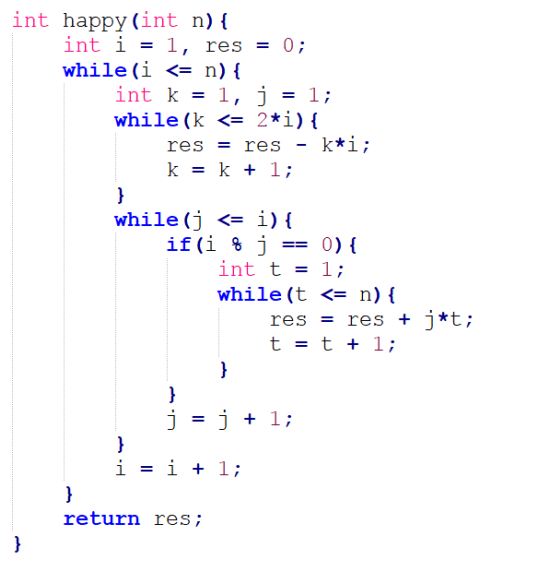
\includegraphics[width=0.5\textwidth]{img1.png} % Đường dẫn tới tập tin hình ảnh
                        \label{fig:hinh_anh}
                    \end{figure}
          \end{enumerate}
          \textbf{Độ phức tạp của đoạn code:}
          \begin{itemize}[label=$\bullet$]
          \item Tổng số phép S : $S=S(Q)=2+\sum_{i \le n} S(P_i)$
          \item $S(P_i) = S(A_{k(i)}) + S(B_{j(i)}) + 1$
          \item Lại có $S(A_{k(i)}) =  2 + 2i + 2i = 4i + 2$
          \item $S(B_{j(i)}) = \sum_{j \le i} ( S(C_{j(i)}) + 1 ) = \sum_{j = 1}^{i} S(C_{j(i)}) + \sum_{j = 1}^{i} 1$
          \item Ta lại có $S(C_{j(i)}) =
    \begin{cases}
        0, & i \not\vdots j \\
        2n+1, & i \vdots j\\
    \end{cases}$
            \item $ S(B_{j(i)}) = \sum_{j; i \not\vdots j} 0 + \sum_{j; i \vdots j} (2n+1) + \sum_{j = 1}^{i} 1 = 0 + (2n+1) \cdot d(i) + i$
            \item $S(P_i) = 3 + 4i + (2n+1) \cdot d(i) + i = 3 + 5i + (2n+1) \cdot d(i)$
          \end{itemize}
          Tính tổng số phép gán:
\[
\begin{aligned}
S &= 2 + \sum_{i = 1}^{n} S(P_i) = 2 + \sum_{i = 1}^{n}(3 + 5i + (2n+1) \cdot d(i)) \\
&= 2 + \sum_{i = 1}^{n} 3 + \sum_{i = 1}^{n}(5i) + \sum_{i = 1}^{n}((2n+1) \cdot d(i)) \\
&= 2 + 3n + 5 \cdot \frac{n(n+1)}{2} + (2n+1) \cdot \sum_{i = 1}^{n}(d(i))
\end{aligned}
\]
Mà ta có: $\sum_{i = 1}^{n}d(i) = d(1)+d(2)+\cdots+d(n) \in \Theta(n \log n)$\\ \\
$ \Rightarrow(2n+1) \cdot \sum_{i = 1}^{n}d(i) \in \Theta(n^2 \log n)$\\ 
\[\Rightarrow S = 2 + 3n + 5 \cdot \frac{n(n+1)}{2} + (2n+1) \cdot \sum_{i = 1}^{n}(d(i)) \in \Theta(n^2 \log n)\]
\textbf{Kết luận:} Độ phức tạp của thuật toán \(\in \Theta(n^2 \log n)\).
\end{enumerate}
\begin{enumerate}[label=\textbf{Câu 2:} ]
    \item Xét đoạn code sau viết bằng C++ để kiểm tra số nguyên dương $a_{0},a_{1},a_{2},\cdots,a_{n-1} $ có thỏa mãn ràng buộc: với mọi $i=0,1,2,\cdots,n-1 $ thì hai số  $a_{i} $ và $i $ đều có cùng tính chẳn lẻ hay không:
          \begin{figure}[h] % Hình ảnh sẽ được đặt tại vị trí gần nhất có thể
              \centering
              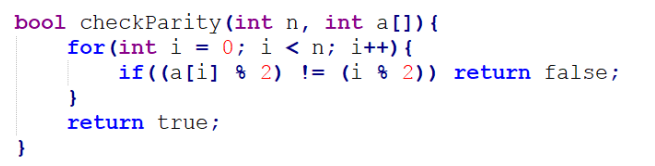
\includegraphics[width=0.5\textwidth]{img2.png} % Đường dẫn tới tập tin hình ảnh
              \label{fig:hinh_anh}
          \end{figure}
          \\
          Giả sử rằng mỗi phần tử của mảng được sinh ngẫu nhiên với xác suất là $\frac{1}{2} $ cho số chẵn và $\frac{1}{2}$ cho số lẻ. Xét $f_{n}(x) $ là hàm sinh xác suất ứng với số lần lặp của thuật toán.
          \begin{enumerate}[label=\alph*)]
              \item CHứng minh rằng $f_{n}(x)=\frac{x}{2}+\frac{x^2}{4}+\frac{x^3}{8}+\cdots+\frac{x^{n-2}}{2^{n-2}}+\frac{x^{n-1}}{2^{n-1}}+\frac{x^{n}}{2^{n}}$\\
              Gọi $P_{k} $ là xác suất vòng lặp dừng lại ở lần thứ k.
              \begin{itemize}[label=$\bullet$]
                \item $1 \leq k\leq n-1:$
                \begin{center}
                    $P_{k}=(\prod_{n = 1}^{k-1}\frac{1}{2})*\frac{1}{2}=(\frac{1}{2})^{k}  $
                \end{center}
                \item k=n:\\
                Vòng lặp bắt buộc phải dừng:
                    $P_{k}=P_{n}=\prod_{n = 1}^{k-1}\frac{1}{2}=(\frac{1}{2})^{k-1}$
              \end{itemize}
              Vậy khi đó hàm sinh xác suất:\\
              \[f_{n}(x)=\sum_{k = 1}^{n}P_{k}x^k=\sum_{k = 1}^{n-1}P_{k}x^k+p_{n}x^n=\sum_{k = 1}^{n-1}(\frac{1}{2})^kx^k+(\frac{1}{2})^{n-1}x^n\]
              \[=\sum_{k = 1}^{n-1}\frac{x^k}{2^k}+\frac{x^n}{2^n-1}=\frac{x^2}{4}+\frac{x^3}{8}+\cdots+\frac{x^{n-2}}{2^{n-2}}+\frac{x^{n-1}}{2^{n-1}}+\frac{x^{n}}{2^{n}}\]
              \item Hãy tính độ phức tạp trung bình của thuật toán bằng cách xác định kỳ vọng của số lần lặp dựa theo hàm sinh trên.\\
              Kỳ vọng của hàm sinh là số lần lặp trung bình của thuật toán hay nói cách khác kỳ vọng của hàm sinh là độ phức tạp trung bình của thuật toán:$ \Leftrightarrow E_{n}(X)=f_{n}'(1)$\\ 
              \[f_{n}'(x)=(\frac{x^2}{4}+\frac{x^3}{8}+\cdots+\frac{x^{n-2}}{2^{n-2}}+\frac{x^{n-1}}{2^{n-1}}+\frac{x^{n}}{2^{n}})'\]
              \[=(\sum_{k = 1}^{n-1}\frac{x^k}{2^k}+\frac{x^n}{2^n-1})'\]
              \[=\sum_{k = 1}^{n-1}\frac{k}{2^k}x^{k-1}+\frac{nx^{n-1}}{2^n-1}\]
              Vậy $E_{n}(X)=f_{n}'(1)=\sum_{k = 1}^{n-1}\frac{k}{2^k}+\frac{n}{2^n-1}=
              \sum_{k = 1}^{n-1}\frac{k}{2^k} + \frac{n}{2^{n-1}}$\\ \\
              Ta sẽ tính toán $S= \sum_{k = 1}^{n-1}  \frac{k}{2^k}$
              \[2S = \sum_{k=1}^{n-1} \frac{2k}{2^k} = \sum_{k=1}^{n-1} \frac{k}{2^{k-1}}= 1 + \sum_{k=2}^{n-1} \frac{k}{2^{k-1}}\]
              \[\Leftrightarrow
                2S  = 1 + \sum_{j=1}^{n-2} \frac{j+1}{2^j} = 1 + \sum_{j=1}^{n-2} \frac{j}{2^j} + \sum_{j=1}^{n-2} \frac{1}{2^j}
                \]
                Ta có:
                \[
                    \sum_{j=1}^{n-2} \frac{1}{2^j} = \frac{1}{2} \left( \frac{1-(\frac{1}{2})^{n-2}}{1-\frac{1}{2}} \right) = 1 - \frac{1}{2^{n-2}}(*)
                \]
                Từ (*)  ta có:
\[
2S = 1 + \sum_{j=1}^{n-2} \frac{j}{2^j} + 1 - \frac{1}{2^{n-2}}=2 + \sum_{j=1}^{n-2} \frac{j}{2^j} - \frac{1}{2^{n-2}}
\]
\[\Leftrightarrow
2S = 2 + S - \frac{n-1}{2^{n-1}}\Leftrightarrow S = 2 - \frac{n-1}{2^{n-1}}
\]
 $\Rightarrow E(X)=2-\frac{n+1}{2^{n-1}}+\frac{n}{2^{n-1}}=2-\frac{1}{2^{n-1}}\in \theta(2)=\theta(1)$\\ 
 Vậy độ phức tạp trung bình của thuật toán là $\theta(1)$
          \end{enumerate}
          \begin{enumerate}[label=\textbf{Câu 3:} ]
              \item Trong bài này, ta sẽ đánh giá độ phức tạp thuật toán bằng thực nghiệm.
                    \begin{enumerate}[label=\alph*)]
                        \item Cài đặt bổ sung các biến đếm số phép S \tikz[baseline] \node[opacity=0.5,anchor=base]{count\_assign}; và số phép so sánh \tikz[baseline] \node[opacity=0.5,anchor=base]{count\_compare}; vào mã nguồn của các thuật toán sau đây,thực hiện đếm rồi lập bảng thống kê hoặc vẽ đồ thị mô tả sự thay đổi của các giá trị đó theo n (SV có thể cài đặt lại bằng Python cũng được,bài làm trên notebook hoặc chụp code chèn vào file báo cáo đều được).
                              \begin{itemize}[label=$\bullet$]
                                  \item Thuật toán tính số Fibonaci dùng đệ quy:
                                        \begin{figure}[h] % Hình ảnh sẽ được đặt tại vị trí gần nhất có thể
                                            \centering
                                            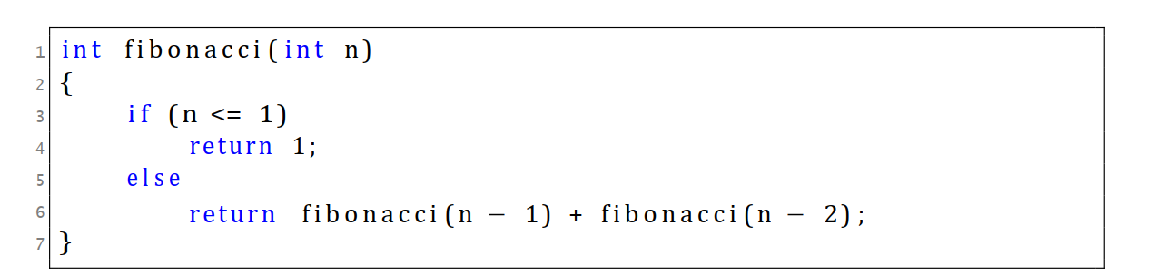
\includegraphics[width=0.5\textwidth]{img3.png} % Đường dẫn tới tập tin hình ảnh
                                            \label{fig:hinh_anh}
                                        \end{figure}
                                    
                                    
                                  \item Thuật toán tính số Fibonaci không đệ quy:
                                        \begin{figure}[h] % Hình ảnh sẽ được đặt tại vị trí gần nhất có thể
                                            \centering
                                            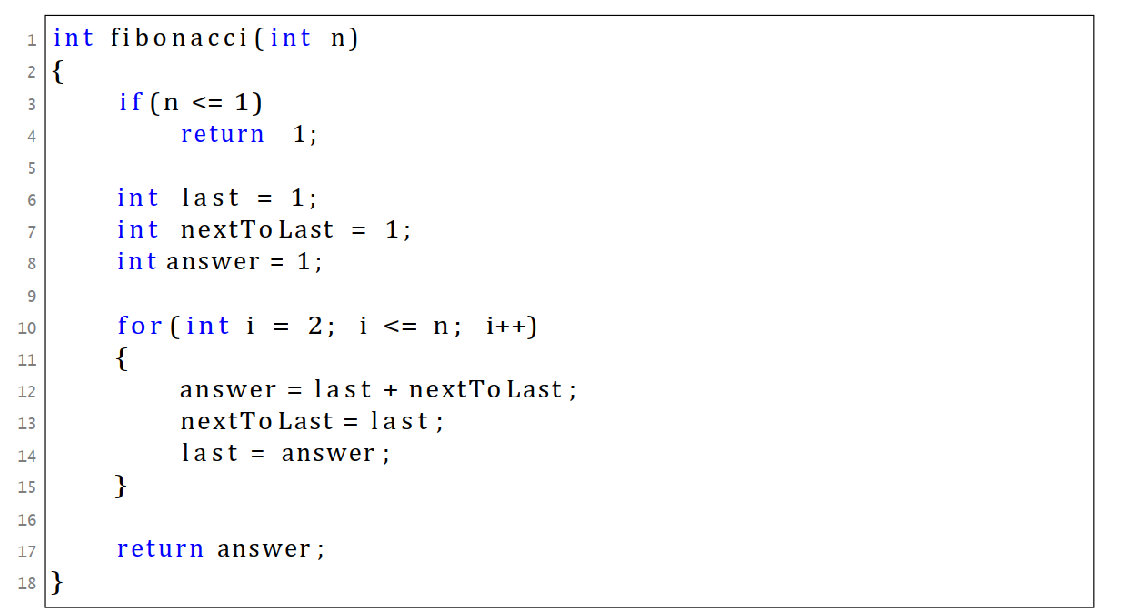
\includegraphics[width=0.5\textwidth]{img4.png} % Đường dẫn tới tập tin hình ảnh
                                            \label{fig:hinh_anh}
                                        \end{figure}
                              \end{itemize}
                              \section*{Thuật toán tính số Fibonaci dùng đệ quy với thêm biến đếm}
                                    Đây là mã nguồn Python triển khai thuật toán Fibonacci dùng đệ quy với các biến đếm số phép gán (assignments) và số phép so sánh (comparisons)\\
                        
                              \begin{lstlisting}
count_assign = 0
count_compare = 0

def fibo(n):
    global count_assign, count_compare
    count_compare += 1
    if n <= 1:
        count_assign += 1
        return n
    count_assign += 1
    return fibo(n - 1) + fibo(n - 2)

# Test with different values of n and store the results
results = []
for n in range(20):  # Change the value in range to test with different n values
    count_assign = 0
    count_compare = 0
    result = fibo(n)
    results.append((n, count_assign, count_compare))

import pandas as pd
import matplotlib.pyplot as plt

# Create the statistics table
df = pd.DataFrame(results, columns=['n', 'count_assign', 'count_compare'])
print(df)

# Plot the graph
plt.figure(figsize=(10, 5))
plt.plot(df['n'], df['count_assign'], label='Number of assignments')
plt.plot(df['n'], df['count_compare'], label='Number of comparisons')
plt.xlabel('n')
plt.ylabel('Number of operations')
plt.title('Number of assignments and comparisons vs. n')
plt.legend()
plt.grid(True)
plt.show()

\end{lstlisting}
\begin{itemize}
    \item \textbf{Kết quả thống kê}\\
    Bảng đây mô tả số phép gán và số phép so sánh cho các giá trị Fibonacci từ 0 đến 9.

\begin{table}[h!]
    \centering
    \begin{tabular}{|c|c|c|}
        \hline
        \textbf{n} & \textbf{Số phép gán} & \textbf{Số phép so sánh} \\
        \hline
        0 & 1 & 1 \\
        1 & 1 & 2 \\
        2 & 2 & 4 \\
        3 & 4 & 8 \\
        4 & 8 & 16 \\
        5 & 14 & 30 \\
        6 & 24 & 52 \\
        7 & 40 & 88 \\
        8 & 66 & 150 \\
        9 & 108 & 256 \\
        10 & 176 & 432 \\
        11 & 286 & 728 \\
        12 & 464 & 1212 \\
        13 & 752 & 1984 \\
        14 & 1218 & 3196 \\
        15 & 1972 & 5128 \\
        16 & 3190 & 8244 \\
        17 & 5164 & 13172 \\
        18 & 8356 & 21092 \\
        19 & 13522 & 33644 \\
        \hline
    \end{tabular}
    \caption{Bảng thống kê số phép gán và số phép so sánh theo n}
\end{table}
\item \textbf{Đồ thị biểu diễn}\\
Đồ thị dưới đây biểu diễn sự thay đổi của số phép gán và số phép so sánh theo giá trị \(n\).
\newpage 
\begin{filecontents*}{data1.dat}
n assign compare
0 1 1
1 1 2
2 2 4
3 4 8
4 8 16
5 14 30
6 24 52
7 40 88
8 66 150
9 108 256
10 176 432
11 286 728
12 464 1212
13 752 1984
14 1218 3196
15 1972 5128
16 3190 8244
17 5164 13172
18 8356 21092
19 13522 33644
\end{filecontents*}

\begin{figure}[h!]
    \centering
    \begin{tikzpicture}
        \begin{axis}[
            xlabel={$n$},
            ylabel={Số phép},
            legend style={at={(0.5,-0.15)},anchor=north,legend columns=-1},
            grid=major,
            width=0.8\textwidth,
            height=0.5\textwidth
        ]
        \addplot table [x=n, y=assign, col sep=space] {data1.dat};
        \addplot table [x=n, y=compare, col sep=space] {data1.dat};
        \legend{Số phép gán, Số phép so sánh}
        \end{axis}
    \end{tikzpicture}
    \caption{Đồ thị số phép gán và số phép so sánh theo n}
\end{figure}
\end{itemize}

\section*{\textbf{Thuật toán tính số Fibonaci không đệ quy với thêm biến đếm}}
                                    Đây là mã nguồn Python triển khai thuật toán Fibonacci không dùng đệ quy với các biến đếm số phép gán (assignments) và số phép so sánh (comparisons)
                        \\
                             \begin{lstlisting}
import matplotlib.pyplot as plt

def fibonacci(n):
    count_assign = 0  # Variable to count assignment operations
    count_compare = 0  # Variable to count comparison operations

    if n <= 0:
        count_compare += 1
        return 0, count_assign, count_compare
    elif n == 1:
        count_compare += 2
        return 1, count_assign, count_compare
    
    count_compare += 2  # Two comparisons are already performed above

    fib_0 = 0
    fib_1 = 1
    count_assign += 2  # Initialize first two values

    for i in range(2, n + 1):
        fib_n = fib_0 + fib_1
        fib_0 = fib_1
        fib_1 = fib_n
        count_assign += 3  # Reassign three values
        count_compare += 1  # Comparison in the loop

    return fib_n, count_assign, count_compare

# Count and plot
n_values = range(1, 21)
assign_counts = []
compare_counts = []

for n in n_values:
    _, count_assign, count_compare = fibonacci(n)
    assign_counts.append(count_assign)
    compare_counts.append(count_compare)

# Plot
plt.figure(figsize=(10, 5))
plt.plot(n_values, assign_counts, label='Number of assignments', marker='o')
plt.plot(n_values, compare_counts, label='Number of comparisons', marker='x')
plt.xlabel('n')
plt.ylabel('Operation Count')
plt.title('Number of assignments and comparisons with n in Fibonacci Algorithm')
plt.legend()
plt.grid(True)
plt.show()
\end{lstlisting}
\begin{itemize}
    \item \textbf{Kết Quả Thống Kê}\\
    Bảng đây mô tả số phép gán và số phép so sánh cho các giá trị Fibonacci từ 0 đến 9.
\begin{table}[h!]
    \centering
    \begin{tabular}{|c|c|c|}
        \hline
        \textbf{n} & \textbf{Số phép gán} & \textbf{Số phép so sánh} \\
        \hline
        0 & 1 & 1 \\
        1 & 1 & 2 \\
        2 & 4 & 3 \\
        3 & 6 & 4 \\
        4 & 8 & 5 \\
        5 & 10 & 6 \\
        6 & 12 & 7 \\
        7 & 14 & 8 \\
        8 & 16 & 9 \\
        9 & 18 & 10 \\
        10 & 20 & 11 \\
        11 & 22 & 12 \\
        12 & 24 & 13 \\
        13 & 26 & 14 \\
        14 & 28 & 15 \\
        15 & 30 & 16 \\
        16 & 32 & 17 \\
        17 & 34 & 18 \\
        18 & 36 & 19 \\
        19 & 38 & 20 \\
        \hline
    \end{tabular}
    \caption{Bảng thống kê số phép gán và số phép so sánh theo n}
\end{table}
\newpage

\begin{filecontents*}{data2.dat}
n assign compare
0 1 1
1 1 2
2 4 3
3 6 4
4 8 5
5 10 6
6 12 7
7 14 8
8 16 9
9 18 10
10 20 11
11 22 12
12 24 13
13 26 14
14 28 15
15 30 16
16 32 17
17 34 18
18 36 19
19 38 20
\end{filecontents*}

\begin{figure}[h!]
    \centering
    \begin{tikzpicture}
        \begin{axis}[
            xlabel={$n$},
            ylabel={Số phép},
            legend style={at={(0.5,-0.15)},anchor=north,legend columns=-1},
            grid=major,
            width=0.8\textwidth,
            height=0.5\textwidth
        ]
        \addplot table [x=n, y=assign, col sep=space] {data2.dat};
        \addplot table [x=n, y=compare, col sep=space] {data2.dat};
        \legend{Số phép gán, Số phép so sánh}
        \end{axis}
    \end{tikzpicture}
    \caption{Đồ thị số phép gán và số phép so sánh theo n}
\end{figure}
\end{itemize}


\item Dùng phương pháp lý thuyết để đếm số phép so sánh được sử dụng ở các câu a) và số phép
                              S được sử dụng ở câu a), xét với n tổng quát (có thể đối chiếu lại với thực nghiệm).
                    \end{enumerate}
          \end{enumerate}
\begin{itemize}
    \item Thuật toán dùng đệ quy:\\
    Gọi $a_n $ là số phép gán của thuật toán fibonaci(n)\\
    Ta có
    $\begin{cases}
        a_0=1,a_0=1 \\
        a_n=a_{n-1}+a_{n-2},n \geq 2\\
    \end{cases}$\\ \\ 
    Đặt $f(z)=\sum_{n = 0}^{+\infty}a_{n}z^n$\\
    Giả sử bán kính hội tụ của $f(z) \text{ là } R>0$\\
\begin{align*}
    f(z) &= \sum_{n=0}^{+\infty} a_n z^n = a_0 z^0 + a_1 z^1 + \sum_{n=2}^{+\infty} (a_{n-1} z^n + a_{n-2} z^n) \\
    &= 1 + z + \sum_{n=2}^{+\infty} (a_{n-1} z^n + a_{n-2} z^n) \\
    f(z) &= 1 + z + z \sum_{n=0}^{+\infty} a_n z^n + z^2 \sum_{n=0}^{+\infty} a_n z^n \\
    f(z) &= 1 + z + z f(z) + z^2 f(z) \\
    f(z) &= 1 + z + f(z)(z + z^2) \\
    f(z) &= \frac{1 - z + z^2}{(1 - z)(1 - z - z^2)} = \frac{1}{1 - z} + \frac{1 - z - z^2}{1 - z} \\
    &= \frac{1}{1 - z} + \frac{-1 + 2z^2}{1 - z - z^2} \\
    &= \frac{1}{1 - z} + \frac{-1}{1 - z} + \frac{2}{1 - z - z^2} \\
    &= \frac{-1}{1 - z} + \frac{2}{1 - z - z^2}
\end{align*}
\[
k(z) = \frac{1}{1-z-z^2} = \frac{1}{(z - \frac{-1 + \sqrt{5}}{2})(z - \frac{-1 - \sqrt{5}}{2})}
\]

\[
\Leftrightarrow k(z) = -\frac{1}{(\frac{-1 + \sqrt{5}}{2} - z)(\frac{-1 - \sqrt{5}}{2} - z)}
\]

\[
\Leftrightarrow k(z) = -\left( \frac{1}{\frac{-1 + \sqrt{5}}{2} \left( 1 - \frac{2}{-1 + \sqrt{5}}z \right)} \right) \left( \frac{1}{\frac{-1 - \sqrt{5}}{2} \left( 1 - \frac{2}{-1 - \sqrt{5}}z \right)} \right)
\]

\[
\Leftrightarrow k(z) = -\left( \frac{1}{-1 + \sqrt{5}} \frac{1}{1 - \frac{2}{-1 + \sqrt{5}}z} \right) \left( \frac{1}{-1 - \sqrt{5}} \frac{1}{1 - \frac{2}{-1 - \sqrt{5}}z} \right)
\]

\[
k(z) = \frac{1}{2} \left( \frac{1}{1 - \frac{2}{-1 + \sqrt{5}}z} \right) \left( \frac{1}{1 - \frac{2}{-1 - \sqrt{5}}z} \right) = \frac{1}{2} \sum_{n=0}^{\infty} \left( \frac{2}{\sqrt{5} - 1}z \right)^n \sum_{n=0}^{\infty} \left( \frac{-2}{\sqrt{5} + 1}z \right)^n
\]

Với \( h(z) = \sum_{n=0}^{\infty} \left( \frac{2}{\sqrt{5} - 1} \right)^n z^n \) và \( g(z) = \sum_{n=0}^{\infty} \left( \frac{-2}{\sqrt{5} + 1} \right)^n z^n \)

\[
k(z) = h(z) \cdot g(z)
\]

Đặt \( k(z) = \sum_{n=0}^{\infty} d_n z^n \)

\[
d_n = \sum_{k=0}^{n} b_k \cdot c_{n-k} = \sum_{k=0}^{n} \left( \frac{2}{\sqrt{5} - 1} \right)^k \left( \frac{-2}{\sqrt{5} + 1} \right)^{n-k}
\]

Ta có:

\[
f(z) = \sum_{n=0}^{\infty} a_n z^n = \frac{-1}{1-z} + \frac{2}{1-z-z^2} = -1 \sum_{n=0}^{\infty} z^n + 2 \sum_{n=0}^{\infty} d_n z^n
\]

Suy ra:

\[
a_n = -1 + d_n = -1 + 2 \sum_{k=0}^{n} \left( \frac{2}{\sqrt{5} - 1} \right)^k \left( \frac{-2}{\sqrt{5} + 1} \right)^{n-k}
\]
\end{itemize}
\end{enumerate}
\end{document}
